\documentclass[a4paper, 12pt]{article}

\usepackage[T1]{fontenc}
\usepackage{booktabs}
\usepackage[toc, page]{appendix}
\usepackage{IEEEtrantools}
\usepackage[]{amsmath}
\usepackage{amssymb}
\usepackage{float}
\usepackage[]{graphicx}
\usepackage{caption}
\usepackage{subcaption}

\title{Control Systems: Practical 4}
\author{216054484 216008466}

\begin{document}

\pagenumbering{gobble}
\maketitle
\newpage
\pagenumbering{roman}
\tableofcontents
\listoffigures
\newpage
\pagenumbering{arabic}

\section{Introduction} % (fold)
\label{sec:introduction}
The purpose of this practical is to model discrete controllers using
approximation methods to convert a continuous controller to a digital
controller  and a more accurate approach where a complete digital design of the
plant and controller is done. Used in this practical is a lead compensator
defined by the equation that follows
\begin{equation}
	\label{eq:lead_compensator}
	D_c(s) = K \frac{Ts + 1}{\alpha Ts + 1}
\end{equation}

where we take $K = 0.28,\,T = 6.7,\,\alpha = 0.106$. This compensator is used
in conjunction with a plant, which in this case, is the simple ball-and-beam
system we have considered in a previous practical. In the previous practical,
we only considered continuous control systems, however, and now we will
investigate how we might implement the same control systems using modern
digital technology. Before we begin, it would be instructive to note the step
response of the plant in series with the lead compensator given in equation
\ref{eq:lead_compensator}, and shown in figure \ref{fig:continuous_control}
below. The rise-time of this system can be found by zooming in on the first
portion of the graph, and we see that it is approximately $t_r = 0.246$
seconds.

\begin{figure}[H]
  \centering
  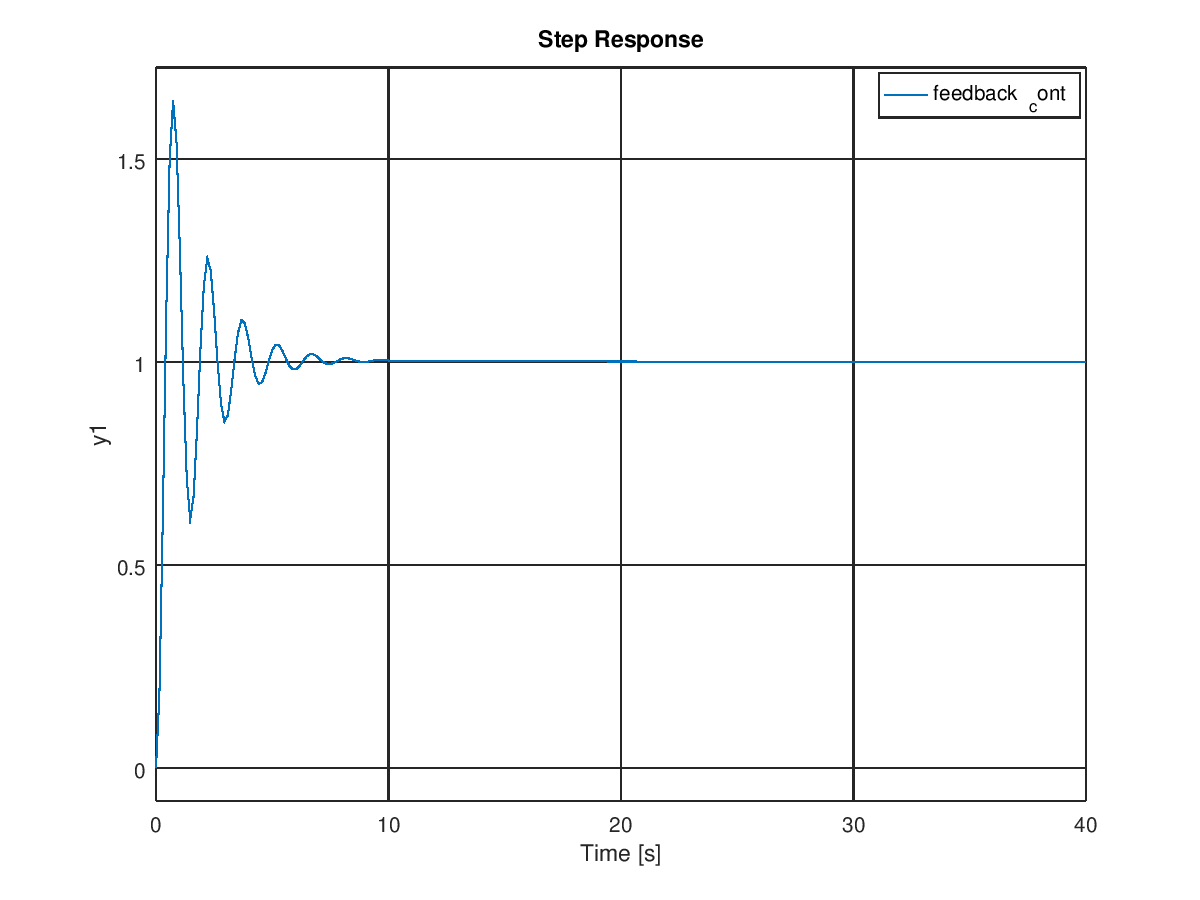
\includegraphics[width=.8\textwidth]{img/continuous_control.png}
  \caption{Continuous control using a lead compensator}
  \label{fig:continuous_control}
\end{figure}
% section introduction (end)

\section{Question 1} % (fold)
\label{sec:question_1}
The Tustin method of approximating the lead controller as defined by equation \eqref{eq:lead_compensator} was used to yield the discrete controller for the system in consideration. To follow are 4 different discrete controller results obtained for a number of different sampling times.

\begin{figure}[H]
  \centering
  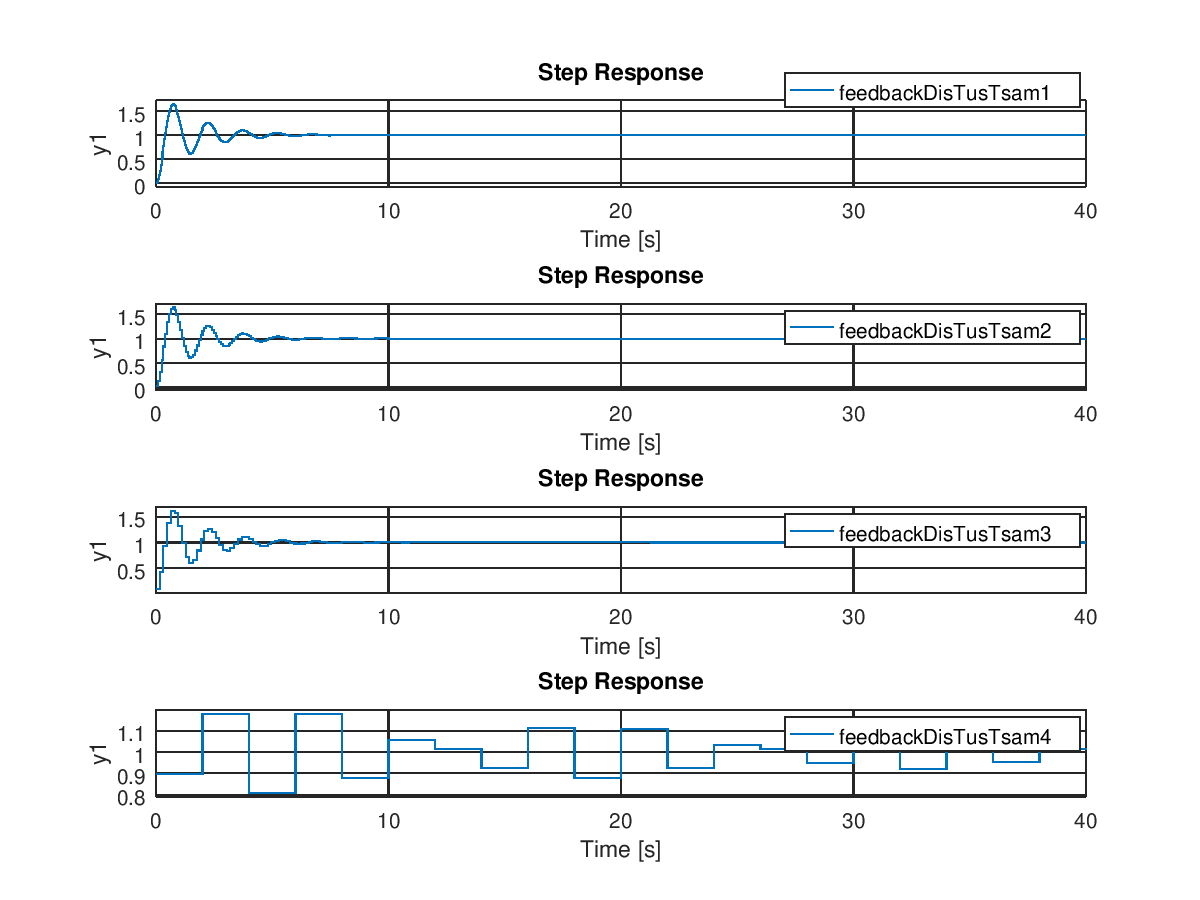
\includegraphics[width=\textwidth]{img/discrete_controllers.png}
  \caption{Discrete control of system using sample times of respectively 0.04, 0.08, 0.16 and 2 seconds}
  \label{fig:discrete_controllers}
\end{figure}

These plots were obtained by running Octave code given in
appendix \ref{sec:appendix_1}. The continuous system was made discrete in order
to implement the feedback using the discrete controllers (another approach that
would yield a better result is to use MATLAB's Simulink)\\

Now comparing these results with the application of the lead compensator, as
dipicted in Figure \ref{fig:continuous_control}, we see that the best discrete
approximation (that lies close to the step response of the continuously
controlled system) is the Tustin discrete controller using a sampling time of
$0.04$ seconds. As the sampling time increases (i.e. less samples are taken
over the course of the same period) the approximation drifts off and the
discrete controller doesn't provided the control that its continuous controller
can provide (and should provide as the discrete controllers are approximations
of the desired system response using a continuous controller).\\

The best sampling time yielding a close to exact replica of a system's response
using a continuous controller is $20\times \omega_n$ where $\omega_n$ is the
natural frequency of the system. Problems with the approximation come into play if the
sampling time is chosen to be $10\times \omega_n$. It is safe to say that using
a sampling time of $2$ seconds, is much less than $10\times \omega_n$ and
sampling times of $0.04$, $0.08$ and $0.16$ lie closer to $20\times \omega_n$




% section question_1 (end)

\section{Question 2}

In this question we try to match the lead compensator's performance from the
previous question, at least in terms of rise-time. We attempt to do this using
the pole placement method. Noticing that our lead compensator exhibits quite a
bit of overshoot, we require the poles of our transfer function to be, first
and foremost, in the left-hand half of the s-plane, but also that the poles
have an imaginary component, which yields the oscillatory motion as seen in
figure \ref{fig:continuous_control}.

By inspection, we find that pole locations of $p = -5 \pm j6$ give a good rise
time along with a good settling time. Sampling at $T = 0.06$ seconds, the step
input of our pole-placement system is given by figure \ref{fig:2_1}.

\begin{figure}[H]
	\centering
	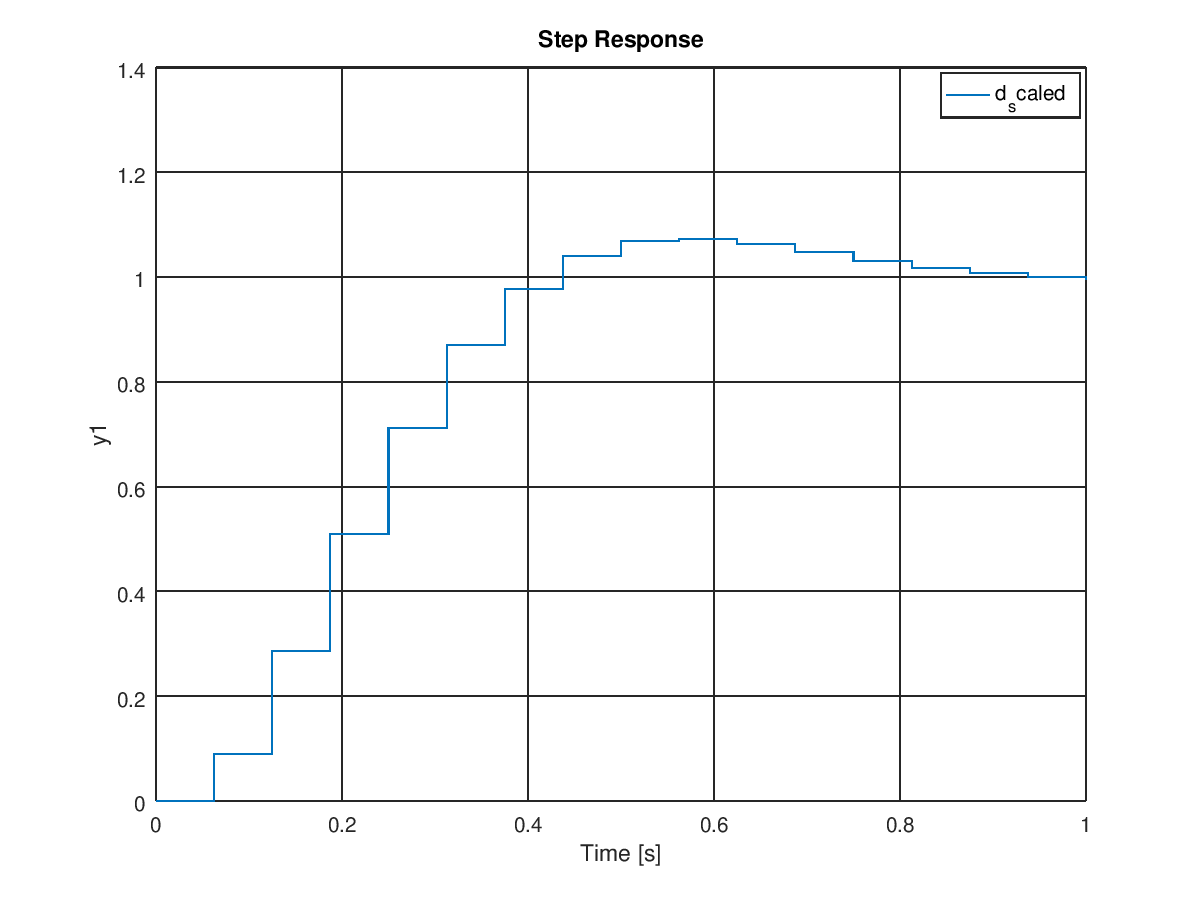
\includegraphics[width=\textwidth]{./img/2_1.png}
	\caption{ZOH system}
	\label{fig:2_1}
\end{figure}

This yields a rise-time of 0.25 seconds, which is very close to the original
rise time of 0.246 seconds. Furthermore, we can show how a reduced sampling
time negatively affects our system's performance in figure \ref{fig:2_2}. Not
only is there a large amount of aliasing taking place, the settling time is
also approximately 1.3 seconds, while the system from figure \ref{fig:2_1}
settles in about 1 second. Clearly, such a long sampling time is not adequate
to control the system. We can explain this from a theoretical observation
called the Nyquist Theorem, which states that we should sample a signal at at
least twice the frequency of the highest frequency component of that signal, if
we are to avoid aliasing distortion effects.

We can also intuitively see this by looking at the unit circle plane of the
z-transform. Since we map the poles with the mapping function $z = e^{sT}$, we
can see that poles having complex components will result in two sinusoidal
components by Euler's formula: $e^{jT} = \cos(T) + j \sin(T)$. The periodicity
of this circle confirms the fact that we need to sample well above our highest
frequency component --- if we do not, then with large values of $T$ frequency
components higher than $\frac{1}{2T}$ will ``wrap around'' the unit circle, and
be indistinguishable from their lower frequency counterparts to the system. In
the context of control systems, it is often advised to sample at a rate of at
least $20 \times \omega_{\text{BW}}$.

\begin{figure}[H]
  \centering
  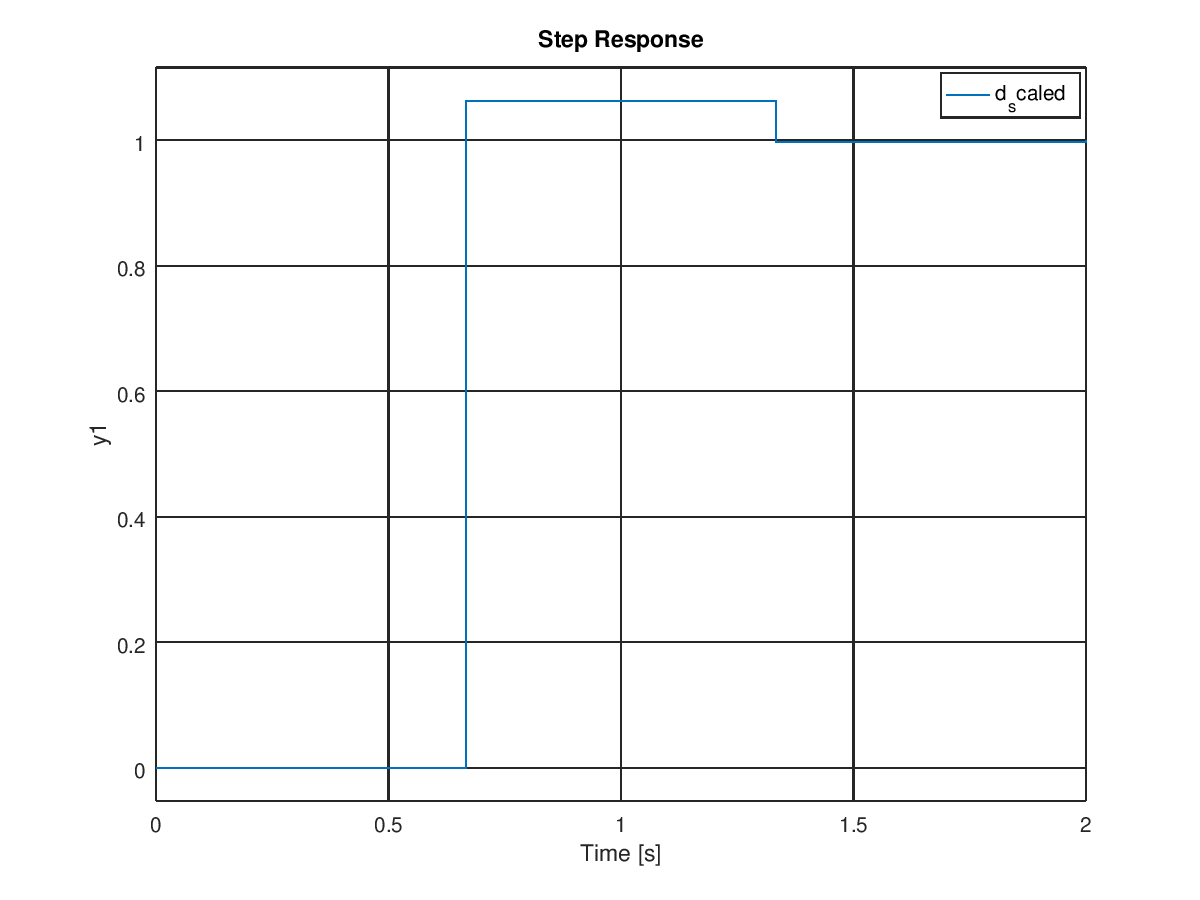
\includegraphics[width=\textwidth]{./img/2_2.png}
  \caption{ZOH system with T = 0.6 seconds}
  \label{fig:2_2}
\end{figure}

% section question_2 (end)

\section{Question 3}

Consider the general control system topology in Figure 8.28, question 2.4 of
the practical assignment. With consideration of the specifications of this
closed loop system, we find the following values that satisfy $\zeta > 0.5$ and
$\omega_n > 1$.

\begin{IEEEeqnarray}{lCl}
  K & = & 5 \label{eq:3_K}\\
  T_D & = & 0.6 \label{eq:3_td} \\
  T_I & = & 1.6667 \label{eq:3_ti}
\end{IEEEeqnarray}

Using the \texttt{damp()} function in Octave, we find that we have the
$\zeta$ and $\omega_n$ values for the system as given in table \ref{tab:specs}.

\begin{table}
  \centering
  \begin{tabular}{c c c c}
    \toprule
    & Pole position & $\zeta$ & $\omega_n$ \\
    \midrule
    $p_1$ & -0.767 + j0.79 & 0.69553 & 1.1031 \\
    $p_2$ & -0.767 + j0.79 & 0.69553 & 1.1031 \\
    $p_3$ & -2.47 & 1.00000 & 2.4656 \\
    \bottomrule
  \end{tabular}
  \caption{Damping ratio and natural frequency attributes of the system}
  \label{tab:specs}
\end{table}

Therefore we get the following negative feedback system, with the step input
response given in figure \ref{fig:2_original}.

\begin{equation}
  G(s) = \frac{3 s^2 + 5s + 3}{s^3 + 4s^2 + 5s + 3}
  \label{eq:gs_original}
\end{equation}

\begin{figure}[H]
  \centering
  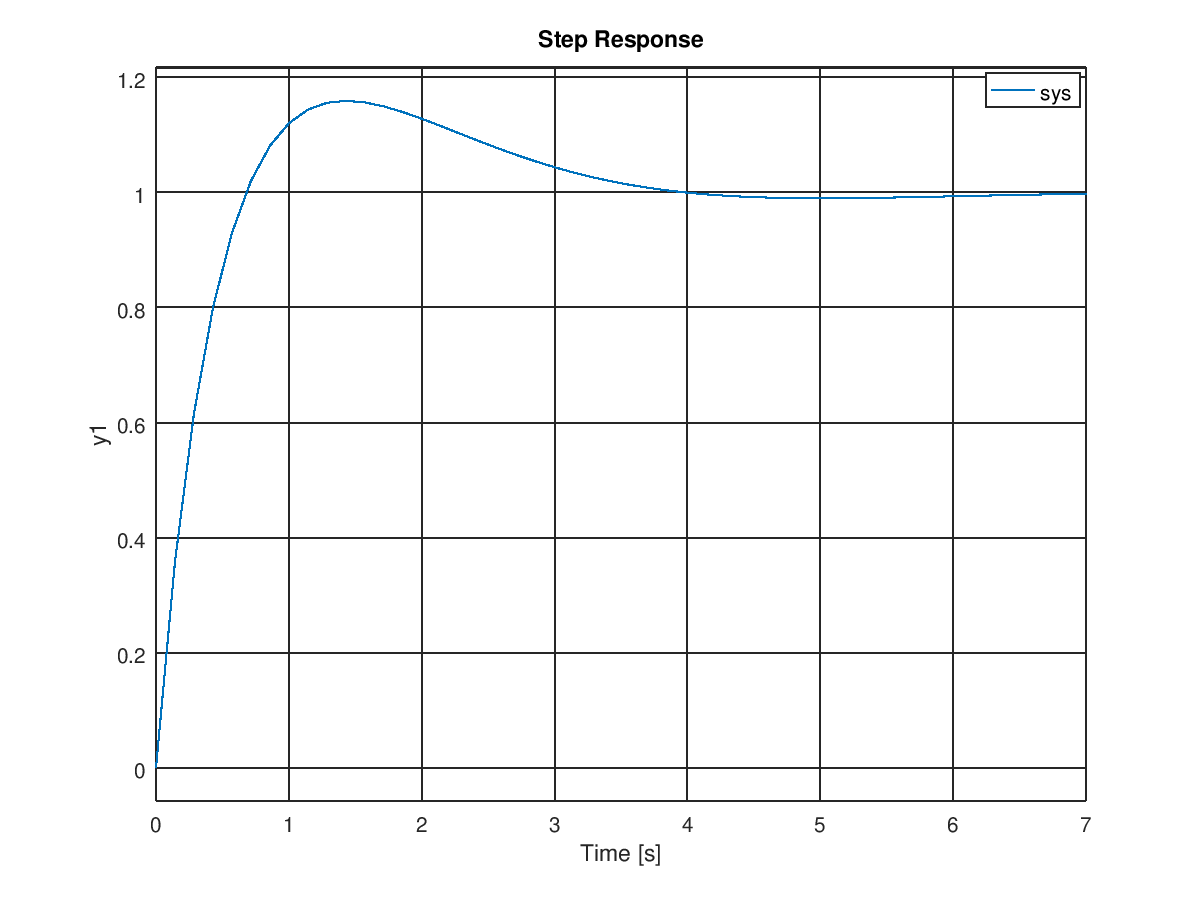
\includegraphics[width=.8\textwidth]{./img/2_5_continuous.png}
  \caption{Step input response of equation \eqref{eq:gs_original}}
  \label{fig:2_original}
\end{figure}

In the following sections, we present the different transfer functions and step
input responses for the discretized controllers based on equation \eqref{eq:gs_original}.\\

% tustin 1
\noindent Tustin's method. Sampling time $T = 1$ second.
\begin{equation}
  G_d(z) = \frac{0.6757 z^3 + 0.1892 z^2 - 0.3514 z + 0.1351}{z^3 - 0.5676 z^2 + 0.1892 z + 0.02703}
  \label{eq:tustin_1}
\end{equation}
% tustin .1
\noindent Tustin's method. Sampling time $T = 0.1$ seconds.
\begin{equation}
  G_d(z) = \frac{0.1343 z^3 - 0.1124 z^2 - 0.1331 z + 0.1137}{z^3 - 2.627 z^2 + 2.299 z - 0.6696}
  \label{eq:tustin_01}
\end{equation}
% tustin .01
\noindent Tustin's method. Sampling time $T = 0.01$ seconds.
\begin{equation}
  G_d(z) = \frac{0.01483 z^3 - 0.01458 z^2 - 0.01483 z + 0.01458}{z^3 - 2.96 z^2 + 2.921 z - 0.9608}
  \label{eq:tustin_001}
\end{equation}
% mpz 1
\noindent Matched Pole-Zero method. Sampling time $T = 1$ second.
\begin{equation}
  G_d(z) = \frac{1.148 z^2 - 0.8495 z + 0.2169}{z^3 - 0.7369 z^2 + 0.271 z - 0.01832}
  \label{eq:mpz_1}
\end{equation}
% mpz .1
\noindent Matched Pole-Zero method. Sampling time $T = 0.1$ seconds.
\begin{equation}
  G_d(z) = \frac{0.2675 z^2 - 0.4916 z + 0.2265}{z^3 - 2.628 z^2 + 2.301 z - 0.6703}
  \label{eq_mpz_01}
\end{equation}
% mpz .01
\noindent Matched Pole-Zero method. Sampling time $T = 0.01$ seconds.
\begin{equation}
  G_d(z) = \frac{0.02965 z^2 - 0.05881 z + 0.02916}{z^3 - 2.96 z^2 + 2.921 z - 0.9608}
  \label{eq:mpz_001}
\end{equation}

To enhance the discussion, the graphs of the step responses have been provided.
Overall, we can see that even though the two different methods tend to yield
dissimilar transfer functions, their characteristics are quite close to one
another. As we can see in figure \ref{fig:tustin001} and figure
\ref{fig:mpz001}, sampling at a very quick rate of 0.01 seconds, we can see
that the discrete system matches the continuous version almost exactly, with no
real appreciable difference. Looking at figures \ref{fig:tustin01} and
\ref{fig:mpz01}, we can now clearly see the reduced resolution by sampling at
0.1 second intervals.  However, the general characteristics seem to have been
preserved in the system.  The overshoot, rise times, and settling times for
both methods seems to have been preserved.

Looking at figure \ref{fig:tustin1} and figure \ref{fig:mpz1} though, we see
that a sampling rate of 1 second seems to drastically affect the discrete
system. The overshoot is drastically increased to more than 25\% for the Tustin
method, and there is clearly a lot of aliasing distortion taking place in both
filter methods, and the reader may refer back to the discussion in the previous
question on why aliasing is detrimental to discrete control systems. The Tustin
method's overshoot can be traced back to the design principles governing it; it
essentially sees discrete control as an integration problem, and uses
trapezoidal integration to perform the discrete transform. This means that,
with a low sampling rate, the errors from this integration process are severe,
particularly before the system reaches steady-state.

\begin{figure}[H]
  \centering
  \begin{subfigure}{.6\textwidth}
    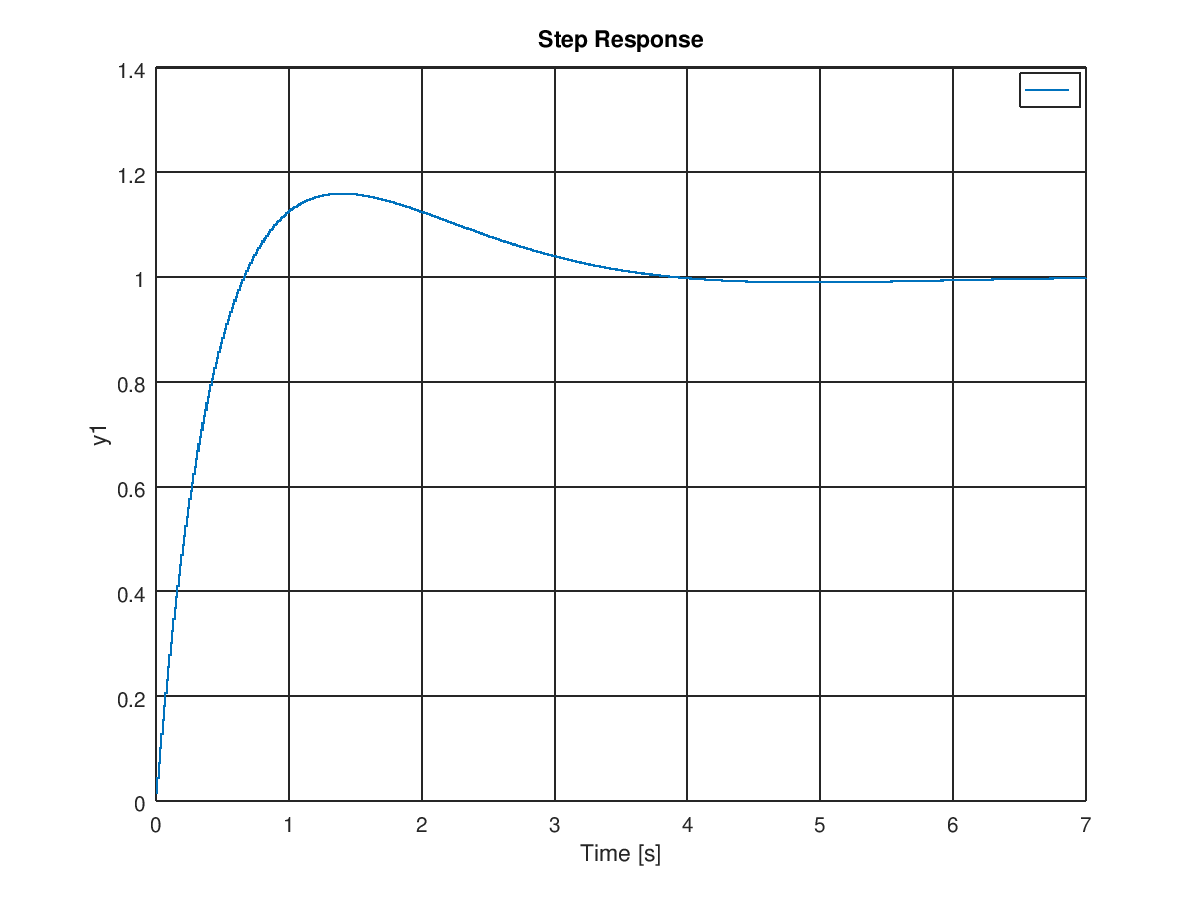
\includegraphics[width=\textwidth]{./img/2_5_tustin001.png}
    \caption{$T = 0.01$ seconds}
    \label{fig:tustin001}
  \end{subfigure}

  \begin{subfigure}{.6\textwidth}
    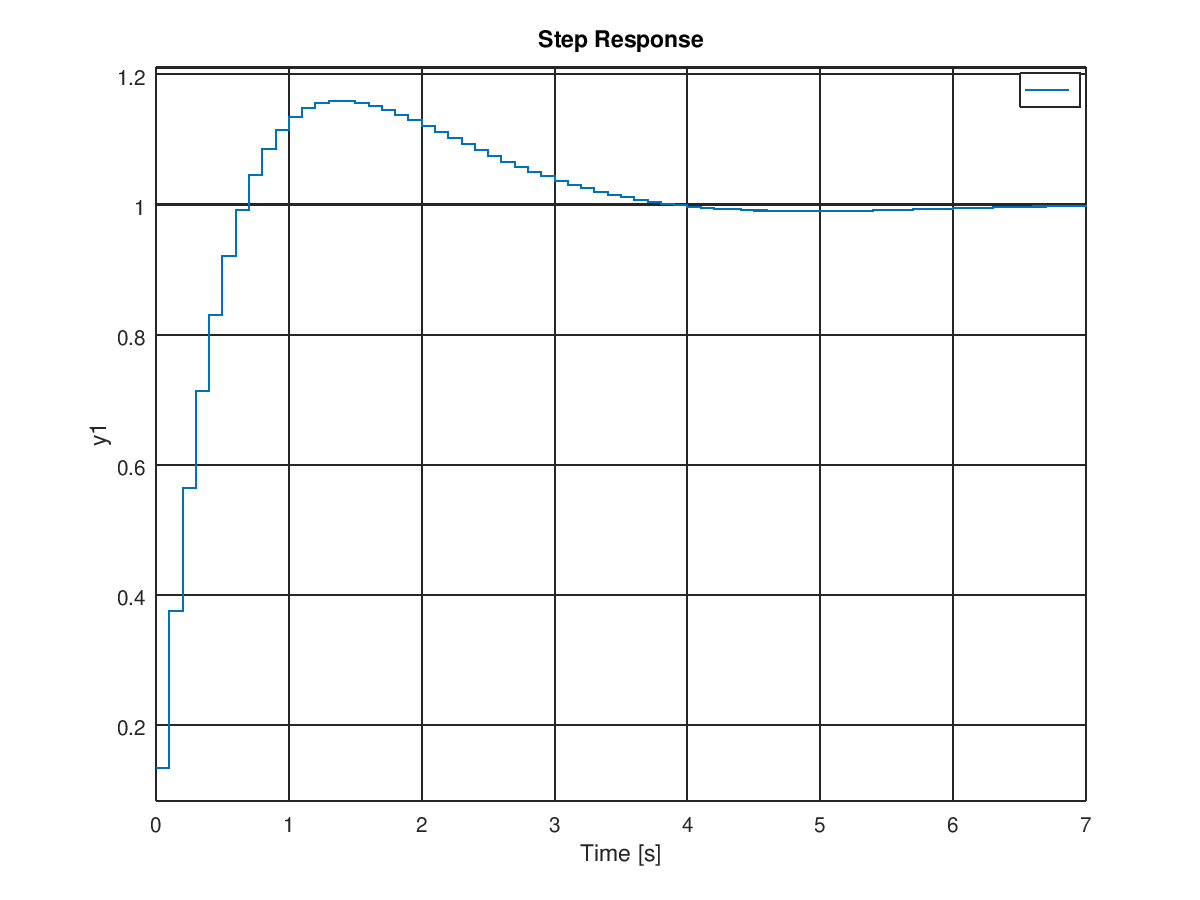
\includegraphics[width=\textwidth]{./img/2_5_tustin01.png}
    \caption{$T = 0.1$ seconds}
    \label{fig:tustin01}
  \end{subfigure}
  
  \begin{subfigure}{.6\textwidth}
    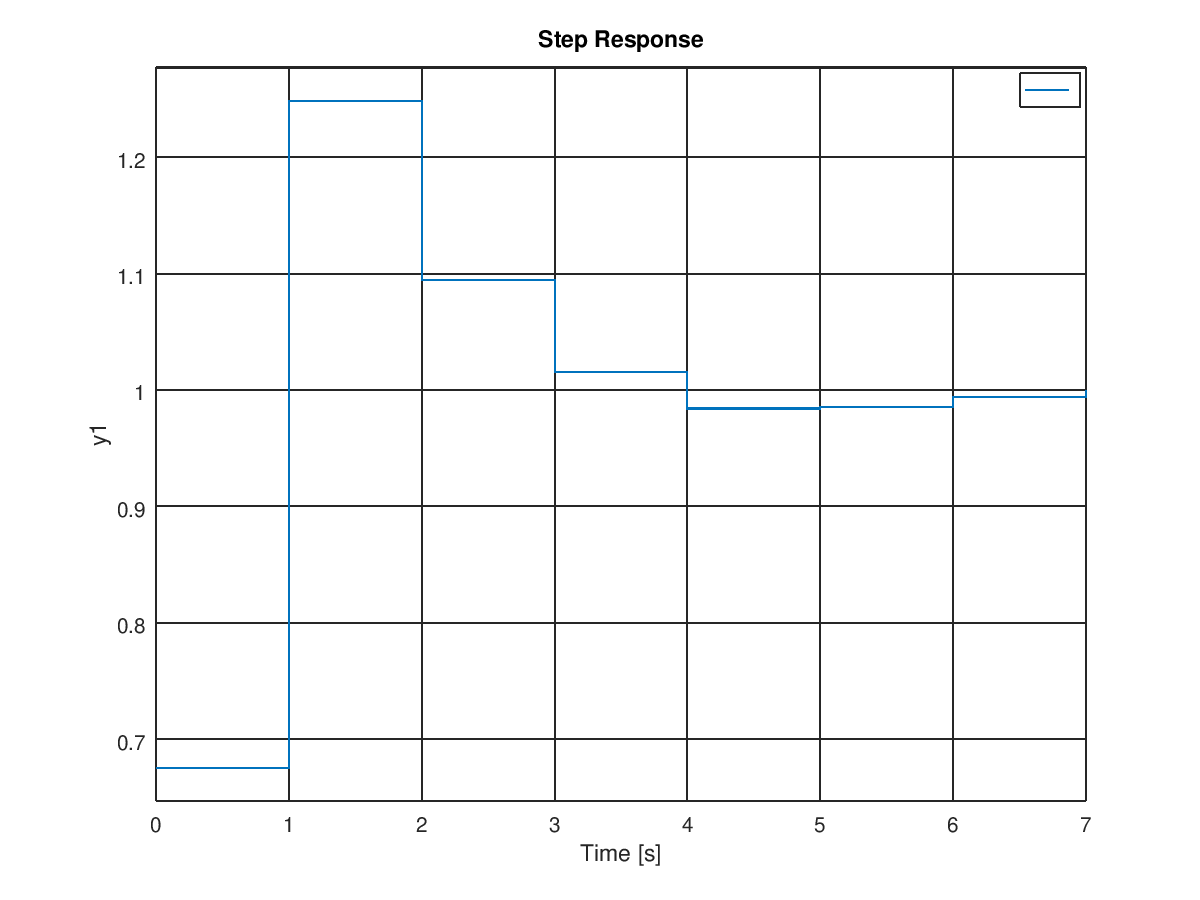
\includegraphics[width=\textwidth]{./img/2_5_tustin1.png}
    \caption{$T = 1$ second}
    \label{fig:tustin1}
  \end{subfigure}
  \caption{Tustin emulation}
\end{figure}

\begin{figure}[H]
  \centering
  \begin{subfigure}{.6\textwidth}
    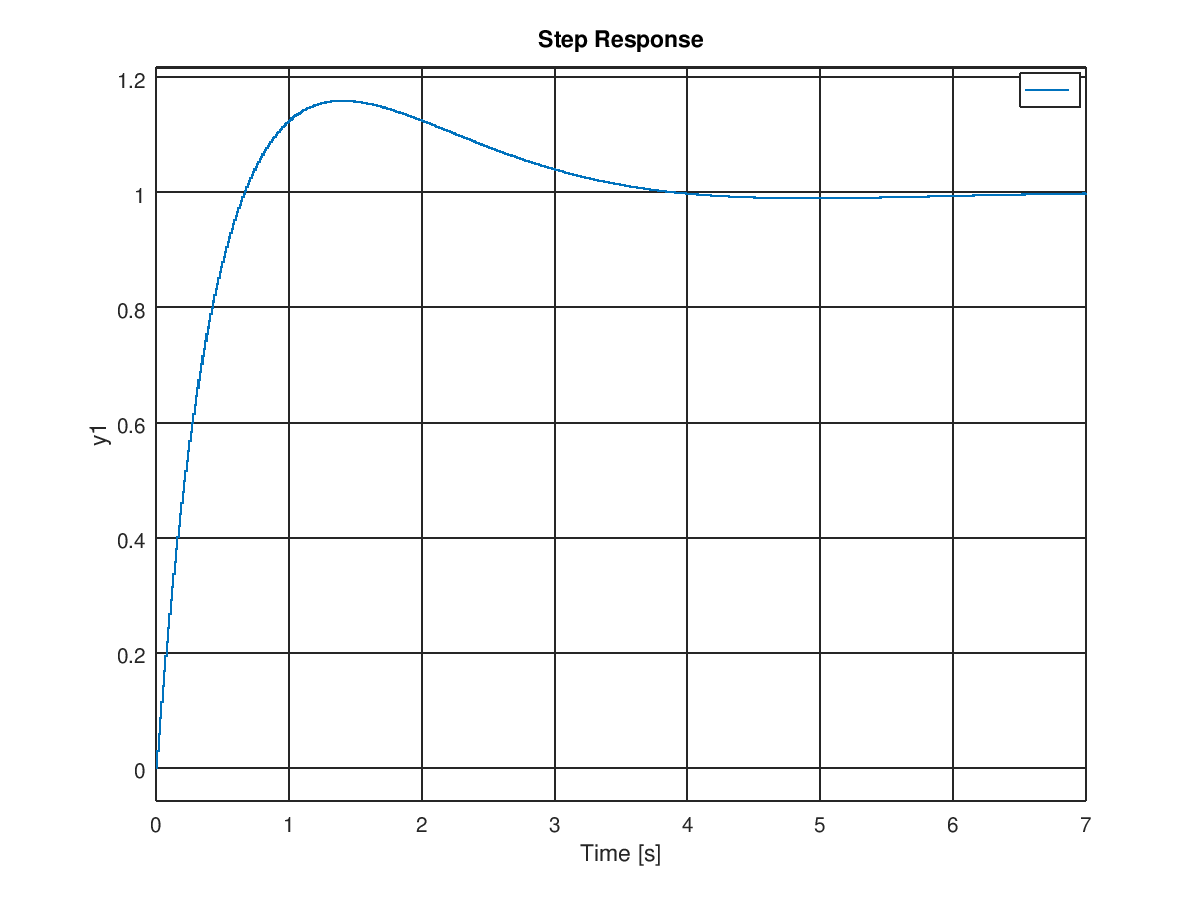
\includegraphics[width=\textwidth]{./img/2_5_mpz001.png}
    \caption{$T = 0.01$ seconds}
    \label{fig:mpz001}
  \end{subfigure}

  \begin{subfigure}{.6\textwidth}
    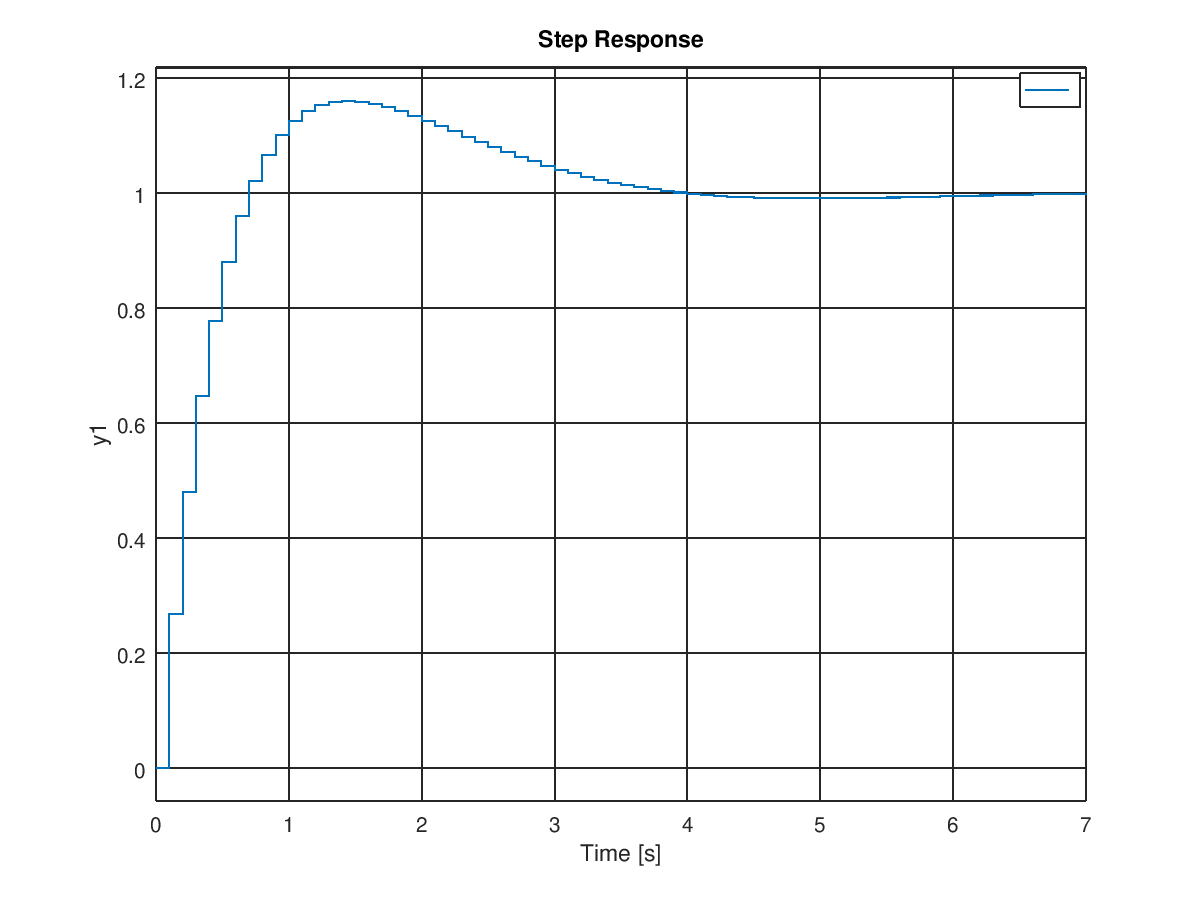
\includegraphics[width=\textwidth]{./img/2_5_mpz01.png}
    \caption{$T = 0.1$ seconds}
    \label{fig:mpz01}
  \end{subfigure}
  
  \begin{subfigure}{.6\textwidth}
    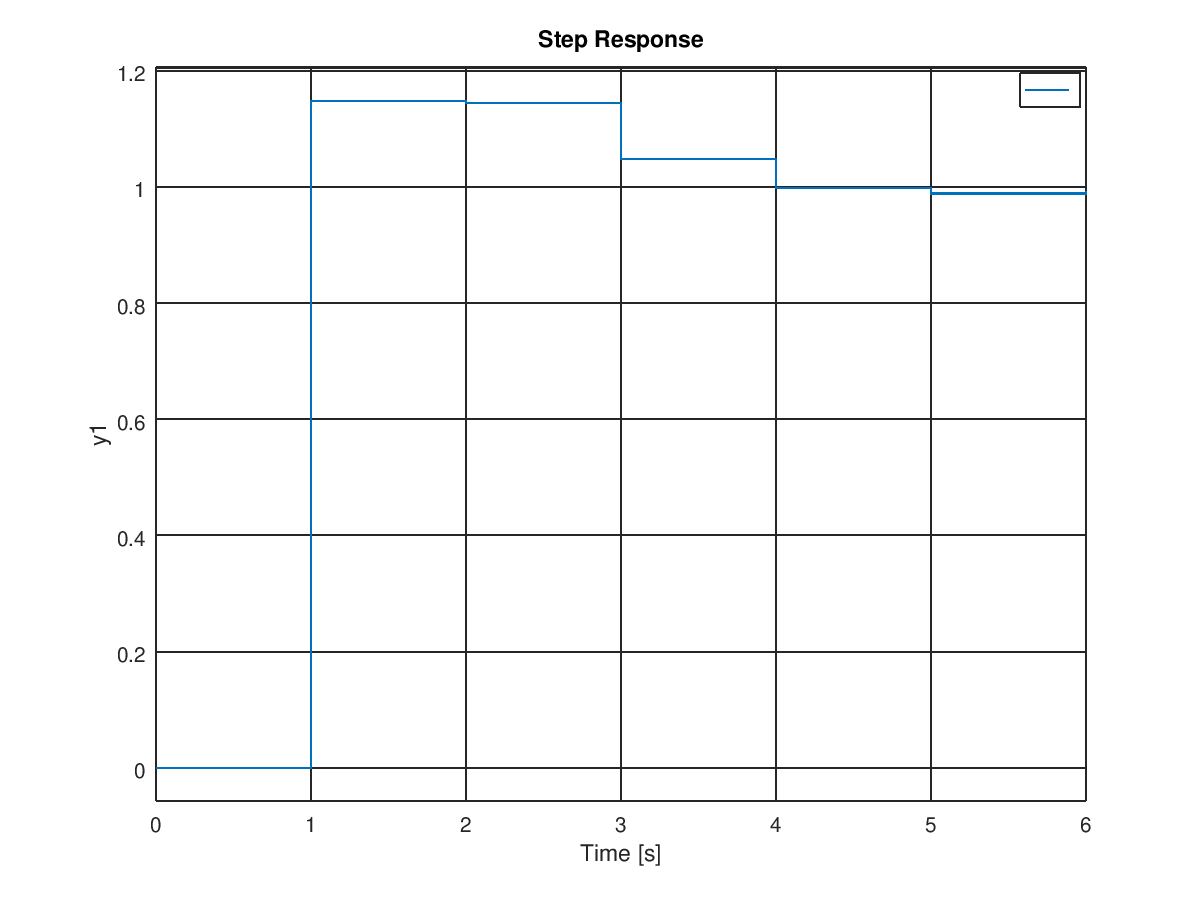
\includegraphics[width=\textwidth]{./img/2_5_mpz1.png}
    \caption{$T = 1$ second}
    \label{fig:mpz1}
  \end{subfigure}
  \caption{Matched Pole-Zero emulation}
\end{figure}
% section question_3 (end)

\begin{appendices}
  \section{Question 1 code}
  \label{sec:appendix_1}
  \noindent
  \texttt{plant = tf([5*9.8],[7 0 0]);}\\
  \texttt{plant\_dis\_tsam1 = c2d(plant,tsam1,'tustin');}\\
  \texttt{plant\_dis\_tsam2 = c2d(plant,tsam2,'tustin');}\\
  \texttt{plant\_dis\_tsam3 = c2d(plant,tsam3,'tustin');}\\
  \texttt{plant\_dis\_tsam4 = c2d(plant,tsam4,'tustin');}\\

  \noindent
  \texttt{cont\_cont = 0.28*tf([6.7 1],[0.106*6.7 1])}\\
  
  \noindent
  \texttt{feedback\_cont = feedback(plant*cont\_cont);}\\
  \texttt{figure;}\\
  \texttt{step(feedback\_cont)}\\
  
  \noindent
  \texttt{dis\_cont\_tus\_tsam1 = c2d(cont\_cont,tsam1,'tustin');}\\
  \texttt{dis\_cont\_tus\_tsam2 = c2d(cont\_cont,tsam2,'tustin');}\\
  \texttt{dis\_cont\_tus\_tsam3 = c2d(cont\_cont,tsam3,'tustin');}\\
  \texttt{dis\_cont\_tus\_tsam4 = c2d(cont\_cont,tsam4,'tustin');}\\
  
  \noindent
  \texttt{feedbackDisTusTsam1 = feedback(plant\_dis\_tsam1*dis\_cont\_tus\_tsam1);}\\
  \texttt{feedbackDisTusTsam2 = feedback(plant\_dis\_tsam2*dis\_cont\_tus\_tsam2);}\\
  \texttt{feedbackDisTusTsam3 = feedback(plant\_dis\_tsam3*dis\_cont\_tus\_tsam3);}\\
  \texttt{feedbackDisTusTsam4 = feedback(plant\_dis\_tsam4*dis\_cont\_tus\_tsam4);}\\
  
  \noindent
  \texttt{figure;}\\
  \texttt{subplot(4,1,1);}\\
  \texttt{step(feedbackDisTusTsam1)}\\
  \texttt{subplot(4,1,2);}\\
  \texttt{step(feedbackDisTusTsam2)}\\
  \texttt{subplot(4,1,3);}
  \texttt{step(feedbackDisTusTsam3)}\\
  \texttt{subplot(4,1,4);}\\
  \texttt{step(feedbackDisTusTsam4)}\\

  \section{Question 2 code}
  \label{sec:appendix_2}
  \texttt{function q22(sampling\_time, pole\_locations)}\\\noindent
  \texttt{\hspace*{1em}  pkg load control;}\\\noindent
  \texttt{\hspace*{1em}  pkg load signal;}\\\noindent
  \texttt{\hspace*{1em}  }\\\noindent
  \texttt{\hspace*{1em}  plant = tf([0 0 7], [1 0 0]);}\\\noindent
  \texttt{\hspace*{1em}  [A, B, C, D] = tf2ss(plant);}\\\noindent
  \texttt{\hspace*{1em}  d\_plant = c2d(plant, sampling\_time);}\\\noindent
  \texttt{\hspace*{1em}  K = place(A, B, pole\_locations);}\\\noindent
  \texttt{\hspace*{1em}  A\_cl = A - B*K;}\\\noindent
  \texttt{\hspace*{1em}  }\\\noindent
  \texttt{\hspace*{1em}  syscl = ss(A\_cl, B, C, D);}\\\noindent
  \texttt{\hspace*{1em}  k\_r = 1/dcgain(syscl);}\\\noindent
  \texttt{\hspace*{1em}  syscl\_scaled = ss(A\_cl, B * k\_r, C, D);}\\\noindent
  \texttt{\hspace*{1em}  d\_scaled = c2d(syscl\_scaled, sampling\_time);}\\\noindent
  \texttt{\hspace*{1em}  step(d\_scaled);}\\\noindent
  \texttt{endfunction}\\\noindent
  \section{Question 3 code}
  \label{sec:appendix_3}
  \texttt{function q25}\\\noindent
  \texttt{\hspace*{1em}  pkg load control;}\\\noindent
  \texttt{\hspace*{1em}  pkg load signal;}\\\noindent
  \texttt{\hspace*{1em}  K =  5;}\\\noindent
  \texttt{\hspace*{1em}  Td =  3 / 5;}\\\noindent
  \texttt{\hspace*{1em}  Ti =  5 / 3;}\\\noindent
  \texttt{\hspace*{1em}  plant = tf([0 0 1], [1 1 0]);}\\\noindent
  \texttt{\hspace*{1em}  s = tf('s');}\\\noindent
  \texttt{\hspace*{1em}  controller = K * (1 + Td * s + 1/(Ti * s));}\\\noindent
  \texttt{\hspace*{1em}  sys = feedback(controller * plant);}\\\noindent
  \texttt{\hspace*{1em}  }\\\noindent
  \texttt{\hspace*{1em}  sampling\_arr = [1, .1, .01];}\\\noindent
  \texttt{\hspace*{1em}  for i = 1:3}\\\noindent
  \texttt{\hspace*{2em}    T = sampling\_arr(i)}\\\noindent
  \texttt{\hspace*{2em}    tustin = c2d(sys, T, 'tustin')}\\\noindent
  \texttt{\hspace*{2em}    mpz = c2d(sys, T, 'mpz')}\\\noindent
  \texttt{\hspace*{1em}  endfor}\\\noindent
  \texttt{endfunction}
\end{appendices}

\end{document}
